\section{Implementazione Behavioural Covert Channel} 
In questo caso ciò che indicherà l'informazione trasmessa, è l'arrivo di un 
determinato messaggio ICMP (la cui tipologia e codice indicano il dato).  
La Figura \ref{fig:behaveCC:eventi:mappatura} mostra come gli eventi vengono 
mappati ai dati trasmessi. 
\vspace{1ex} \newline 
Siccome la quantità di messaggi possibili risulta 17;  
ogni evento permetterà di codificare 4 bit alla volta\footnote{
    $\log_216=4$
}. 
L'evento che rimane inutilizzato, verrà usato per indicare l'inizio e la 
terminazione dell'invio dei dati. 
\vspace{3ex}\newline
\begin{minipage}{\textwidth}
    \centering
    \captionof{figure}{Schema Behavioural Channel  \cite{francesco_santini}\cite{draw_io}} 
    \label{fig:behaveCC:eventi:mappatura}
    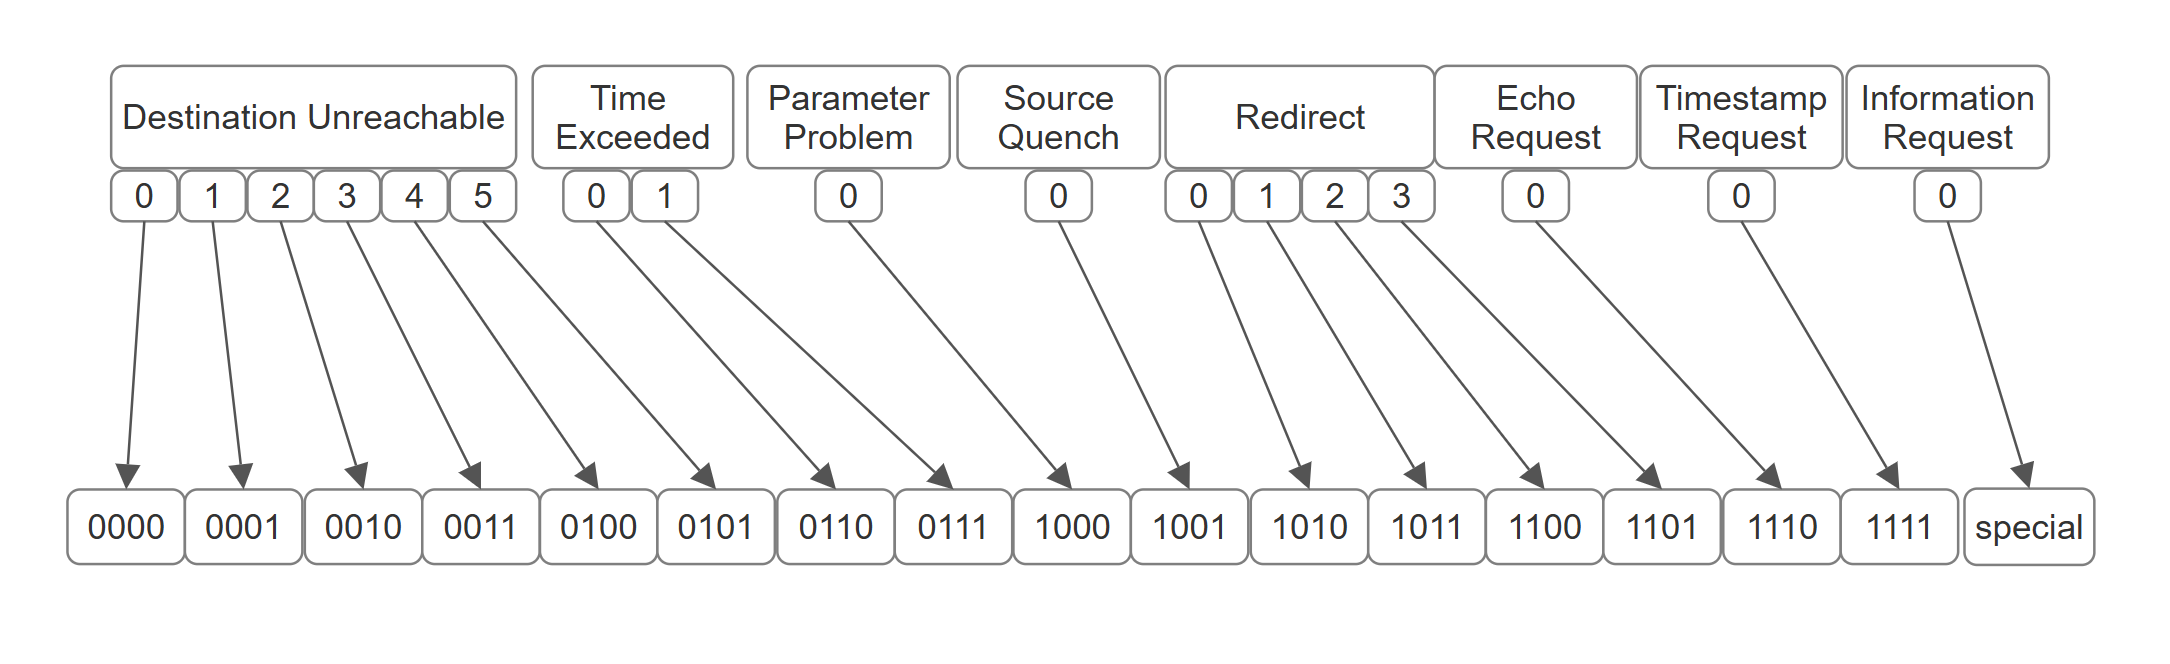
\includegraphics[width=\textwidth]{./img/ICMP_behaveCC/behavioural_channel_1.png}
\end{minipage}  
\vspace{1ex} \newline 
Siccome un singolo evento può trasmettere solo 4 bit; l'invio di un byte, 
prevede la sua divisione in due parti. 
Quindi i primi quattro bit ricavati (così come gli ultimi quattro), 
determineranno la tipologia ed il codice del messaggio da inviare.   
La Figura \ref{listing:behaveCC:divisionebyte} mostra questo processo.  
\begin{lstlisting} 
data='m' 
data.hex=0x6D
data.bytes=b'0110 1101'

Maschera il byte con b'11110000' per ottenere: 0x60 
Shift a destra di 4 bit per ottenere: 0x06 
I primi 4 bit sono: 0110

Maschera il byte con b'00001111' per ottenere: 0x0D
Gli ultimi 4 bit sono: 1101

Mappa b'0110' alla tipologia ed al codice:
    Tipologia: Time Exceeded (tipo 11)
    Codice: 0 (Time to Live exceeded in Transit)
Mappa b'1101' alla tipologia ed al codice:
    Tipologia: Redirect (tipo 5)
    Codice: 3 (Redirect for the host)

Invia un messaggio ICMP Time Exceeded con codice 0
Invia un messaggio ICMP Redirect con codice 3
\end{lstlisting}
\captionof{figure}{Esempio dell'invio di un byte tramite due eventi}
\label{listing:behaveCC:divisionebyte} 
\vspace{2ex} 
Il destinatario, per ricavare i dati, monitora il traffico di rete e controllerà le tipologie di 
messaggi ICMP ricevuti; per ognuno di essi, prende la coppia (Tipologia, Codice) e da questa 
ricaverà i quatttro bit associati. 

\subsubsection{Tipologie di messaggi deprecati} 
Un problema di questa possibile implementazione, sono le tipologie deprecate 
dei messaggi. Questi messaggi potranno comunque essere inviati ma le linee 
guida \cite{icmp_deprecated}\cite{rfc6918_deprecated_types}\cite{rfc6633_sourcequench} 
indicano ai router di ignorarli e all'host utente di non mandarli.  
\vspace{1ex} \newline 
L'uso di tipologie deprecate renderà quindi il canale meno legittimo e più 
facile da individuare. Inoltre, siccome questo tipo di traffico sarà visto 
con sospetto, non è assicurata la ricezione dei messaggi. 


\subsubsection*{Source Quench} 
Il messaggio ICMP Source Quench (tipo 4, codice 0) era concepito come meccanismo per il controllo della congestione. 
Tuttavia, data la sua inefficacia per la congestione, la generazione di questi messaggi da parte dei router è 
stata formalmente deprecata dal 1995. %\cite{rfc1812}.  
Per questo la maggior parte delle implementazioni TCP ignorano silenziosamente i messaggi ICMP Source Quench. 
Infatti TCP implementa i propri meccanismi di controllo della congestione (che non dipendono dai messaggi ICMP Source Quench). 
\vspace{1ex} \newline 
Quindi, siccome la reazione a questi messaggi nei protocolli di trasporto non è mai stata formalmente deprecata, 
la IETF (Internet Engineering Task Force) ha aggiornato le linee guida riguardo il messaggio Source Quench in questo modo:  
\begin{itemize}
    \item Un host \textbf{NON DEVE inviare} dei messaggi di questo tipo. 
    Se viene ricevuto un messaggio di questo tipo, \textbf{PUÒ ignorarlo} (silenziosamente). 
    \item Un router \textbf{DEVE ignorare} tutti i messaggi ICMP Source Quench ricevuti. 
    Inoltre \textbf{NON DOVR\uppercase{à} inviare} messaggi ICMP Source Quench in risposta a una congestione. 
    \item Se un protocollo di trasporto riceve un messaggio Source Quench, \textbf{DEVE essere ignorato/scartato} silenziosamente. 
    \item Host, gateway e firewall DEVONO scartare silenziosamente i pacchetti ICMP Source Quench 
    ricevuti e \textbf{DOVREBBERO registrare} la cosa come un errore di sicurezza con almeno i seguenti dettagli 
    (indirizzo IP sorgente, indirizzo IP di destinazione, tipo di messaggio ICMP, data/ora in cui il pacchetto 
    è stato visualizzato). 
\end{itemize} 
Nell'Internet attuale, non ci sono ragioni per cui un host debba generare o reagire a un messaggio ICMP Source Quench %nell'attuale Internet. 
(o perchè un router debba reagire).  
L'unico motivo per cui un utente ignori questo requisito, è per poter consumare le risorse di rete. %e di endpoint.
I messagg ICMP Source Quench potrebbero essere infatti sfruttati per eseguire attacchi "blind throughput-reduction". 
Le linee guida indicano di ignorare silenziosamente questi messaggi; questo eliminerà il vettore di attacco. 
\vspace{1ex} \newline 
Inoltre, siccome la generazione e la reazione ai messaggi ICMP Source Quench è stata deprecata, le applicazioni 
non dovranno aspettarsi di ricevere questi messaggi. 

\subsubsection*{Information Request/Reply} 
\uppercase{è} stato deprecato siccome meccanismi come il DHCP \cite{rfc2131_DHCP}, lo hanno sostituito per la configurazione dell'host
